\documentclass[t]{beamer}
\usefonttheme{serif}

\usepackage{amsmath,amsthm,amssymb,amsfonts,amscd,mathrsfs,amsxtra,multirow,kotex,mathtools,gensymb,textcomp,lipsum,tikz,verbatim,color,soul,courier,mdframed,xcolor}
\usepackage[normalem]{ulem}
\usetikzlibrary{calc,matrix,arrows,chains,positioning,scopes}
\usepackage{pdfpages}

\theoremstyle{plain}
\newtheorem{thm}{Theorem}[section]
\newtheorem{prop}[thm]{Proposition}

\theoremstyle{definition}
\newtheorem{defn}[thm]{Definition}
\newtheorem{exmp}[thm]{Example}
\newtheorem{excs}[thm]{Exercise}
\newtheorem{rem}[thm]{Remark}
\newtheorem{prob}[thm]{Problem}
\newtheorem{cor}[thm]{Corollary}

\newcommand \tr[1]{\textcolor{red}{#1}}
\newcommand{\tikzmark}[1]{\tikz[overlay,remember picture] \node (#1) {};}
\newcommand{\varep}{\varepsilon}
\newcommand{\DrawBox}[1][]{%
    \tikz[overlay,remember picture]{
    \draw[red,#1]
      ($(left)+(-0.2em,0.9em)$) rectangle
      ($(right)+(0.2em,-0.3em)$);}
}

\newcommand{\tikzmarkk}[2]{
    \tikz[overlay,remember picture,baseline] 
    \node[anchor=base] (#1) {$#2$};
}
\newcommand*\circled[1]{\tikz[baseline=(char.base)]{
            \node[shape=circle,draw,inner sep=2pt] (char) {#1};}}

\tikzset{join/.code=\tikzset{after node path={%
\ifx\tikzchainprevious\pgfutil@empty\else(\tikzchainprevious)%
edge[every join]#1(\tikzchaincurrent)\fi}}}

\tikzset{>=stealth',every on chain/.append style={join},
         every join/.style={->}}
\tikzstyle{labeled}=[execute at begin node=$\scriptstyle,
   execute at end node=$]

\newenvironment<>{proofs}[1][\proofname]{%
   \par
   \def\insertproofname{#1\@{.}}%
   \usebeamertemplate{proof begin}#2}
 {\usebeamertemplate{proof end}}
 

\addtobeamertemplate{navigation symbols}{}{%
    \usebeamerfont{footline}%
    \usebeamercolor[fg]{footline}%
    \hspace{1em}%
    \raisebox{2pt}[0pt][0pt]{\insertframenumber/\inserttotalframenumber}
}
\setbeamercolor{footline}{fg=blue}
\setbeamerfont{footline}{series=\bfseries}
\title[]{SE102:Multivariable Calculus}

\author[]{Hyosang Kang\inst{1}}

\institute[]{\inst{1}Division of Mathematics\\ School of Interdisciplinary Studies\\ DGIST}

\date[]{Lecture 04\\
Maxima and Minima}

\begin{document}

\begin{frame}
\titlepage
\end{frame}

\begin{frame}
\begin{defn}
An \textbf{open ball} $B_{\varepsilon}(\mathbf a)$
of the radius $\varepsilon>0$
at a point $\mathbf a \in\mathbf R^n$
is the set defined by
\[B_{\varepsilon}(\mathbf a) 
= \{\mathbf x\in\mathbf R^n \,|\,
    \Vert\mathbf x-\mathbf a\Vert<\varepsilon\}\]
\end{defn}
\begin{defn}
A function $f(x_1,\ldots,x_n) = (y_1,\ldots,y_m)$
is said to be \textbf{continuously differentiable},
or of \textbf{class $\mathcal C^1$}, at $\mathbf a\in\mathbf R^n$
if there is $\varepsilon >0$ such that 
all the partial derivatives 
$\displaystyle\frac{\partial y_j}{\partial x_i}$
are continuous on an open ball $B_\varepsilon(\mathbf a)$.
\end{defn}
\end{frame}

\begin{frame}
\begin{thm}
If a function $z = f(x,y)$ is continuously differentiable
at $\mathbf a = (x_0,y_0)$, then it is differentiable at $\mathbf a$.
\end{thm}
\begin{proofs}
Let $B_\varepsilon(\mathbf a)$ be an open ball on
which the partial derivatives $f_x,f_y$ are continuous.
Let us choose a point 
$\mathbf b = (x,y) \in B_\varepsilon(\mathbf a)$
and define a sequence 
\[\mathbf p_0 = \mathbf a, \quad 
\mathbf p_1 = (x, y_0), \quad
\mathbf p_2 = \mathbf b\]
Without loss of generality, we will assume that 
$x_0\le x$ and $y_0\le y$.
Define a function $\phi_1(t) = f(t, y_0)$ on $[x_0, x]$.
Note that $\phi_1'(t) = f_x(t,y_0)$.
By the mean value theorem on one-variable function,
there is $t_1\in[x_0,x]$ such that 
\[\phi_1'(t_0)(x-x_0) = f(x,y_0) - f(x_0,y_0)\]
\end{proofs}
\end{frame}

\begin{frame}
\begin{proofs}
Likewise, let us define $\phi_2(t) = f(x,t)$ on $[y_0,y]$,
then there exists $t_2\in[y_0,y]$ satisfying
\[\phi_2'(t_2)(y-y_0) = f(x,y) - f(x,y_0)\]
Then,
\begin{align*}
&f(\mathbf b) - f(\mathbf a) 
    - f_x(\mathbf a)(x-x_0) - f_y(\mathbf a)(y-y_0)\\
&= (\phi_1'(t_1) - f_x(\mathbf a))(x - x_0)
    + (\phi_2'(t_2) - f_y(\mathbf a))(y - y_0)\\
&= (f_x(t_1,y_0) - f_x(\mathbf a))(x - x_0)
    + (f_y(x,t_2) - f_y(\mathbf a))(y - y_0)\\
\end{align*}
Note that as $\mathbf b\to\mathbf a$, we have
$t_1\to x_0$ and $t_2\to y_0$, which means 
the above goes to $0$. 
Since $(x-x_0)/\Vert\mathbf b-\mathbf a\Vert$ and 
$(y-y_0)/\Vert\mathbf b-\mathbf a\Vert$ bounded,
we proved the differentiability of $f$ at $\mathbf a$. 
\end{proofs}
\end{frame}

\begin{frame}
\begin{defn}
A function $z = f(x,y)$ is said to be of 
\textbf{class $\mathcal C^2$} at $\mathbf a\in\mathbf R^2$
if there exists $\varepsilon>0$ such that
all second-order partial derivatives are continuous 
on an open ball $B_\varepsilon(\mathbf a)$.
\end{defn}
\begin{rem}
Given a function $\mathbf f:\mathbf R^n\to\mathbf R^m$,
the derivative $\mathbf{Df}$ is a function 
$\mathbf{Df}:\mathbf R^n\to\mathbf R^{nm}$
whose coordinate functions are all the first derivatives of
$\mathbf f$.
The function $\mathbf f$ being a class $\mathcal C^1$ 
means that $\mathcal{Df}$ is continuous.
Similarly, being a class $\mathcal C^2$ means that
$\mathbf{Df}$ is $\mathcal C^1$, 
which equivalent to saying that $\mathbf D^2\mathbf f$ is continuous.
We say the function $\mathbf f$ is of class $\mathcal C^n$
if $\mathbf D^n\mathbf f$ is continuous.
Moreover, the function $\mathbf f$ is of class $\mathcal C^\infty$
if $\mathbf D^n\mathbf f$ is continuous for all $n>0$.
\end{rem}
\end{frame}

\begin{frame}
\begin{thm}[Clairaut]
If $z = f(x,y)$ is of class $\mathcal C^2$ at $(x_0,y_0)$, then
\[f_{xy}(x_0,y_0)=f_{yx}(x_0,y_0).\]
\end{thm}

\begin{exmp}
Check if the following function satisfies 
Clairaut's theorem at $(0,0)$.
\[f(x,y)=\begin{dcases}
xy\frac{x^2-y^2}{x^2+y^2}&(x,y)\neq(0,0)\\
0& (x,y)=(0,0)
\end{dcases}\]
\end{exmp}
\end{frame}

\begin{frame}
\begin{proofs}[Proof of Clairaut's Theorem]
Let us define $\mu: B_\varepsilon(\mathbf a)\to\mathbf R$ as 
\[\mu(x,y) = f(x,y) - f(x_0,y) - f(x,y_0) + f(x_0,y_0)\]
Let us define $\phi(t) = f(t,y) - f(t,y_0)$ on $[x_0,x]$.
Since $f$ is of class $\mathcal C^1$, 
$\phi$ is differentiable on $[x_0, x]$.
Note that 
\[\mu(x,y) = \phi(x) - \phi(x_0).\] 
By the mean value theorem, there exists
$t_1\in[x_0,x]$ satisfying
\[\mu(x,y) = \phi'(t_1)(x-x_0) = (f_x(t_1,y) - f_x(t_1,y_0))(x-x_0).\]
Since $f_x$ is of class $\mathcal C^1$, 
we can apply the mean value theorem on 
$\psi(h) = f_x(t_1,h)$, which means that
there exists $t_2\in[y_0, y]$ satisfying
\[f_x(t_1,y) - f_x(t_1,y_0) = \psi'(t_2)(y-y_0) 
= f_{xy}(t_1,t_2)(y-y_0)\]
\end{proofs}
\end{frame}

\begin{frame}
\begin{proofs}
Thus we showed that there exists 
$(t_1,t_2)\in[x_0,x]\times[y_0,y]$ satisfying
\[\mu(x,y) = f_{xy}(t_1,t_2)(x-x_0)(y-y_0).\]
If we switch the role of $x$ and $y$ when we defined $\phi$,
we would obtain the similar result:
there exists a point $(s_1,s_2)\in[x_0,x]\times[y_0,y]$
satisfying
\[\mu(x,y) = f_{yx}(s_1,s_2)(x-x_0)(y-y_0).\]
Let us replace $x= x_0+h$ and $y=y_0+h$. 
Since we assume that $f$ is of class $\mathcal C^2$,
the following function converges as $(x,y)\to(x_0,y_0)$.
\[\frac{\mu(x_0+h,y_0+h)}{h^2} 
    = f_{xy}(t_1,t_2) = f_{yx}(s_1,s_2)\]
Since $(t_1,t_2),(s_1,s_2)\to(x_0,y_0)$ as $(x,y)\to(x_0,y_0)$,
we are done.
\end{proofs}
    
\end{frame}
\begin{frame}
\begin{defn}
Suppose that $f(x,y)$ is of class $\mathcal C^2$ at $(x_0,y_0)$.
Then the following polynomial 
is called the \textbf{Taylor polynomial of second degree $2$}
of $f$ at $(x_0,y_0)$.
	\begin{align*}
	Q(&x,y)= f(x_0,y_0)+f_x(x_0,y_0)(x-x_0)\\
	&+f_y(x_0,y_0)(y-y_0)+\frac{1}{2}f_{xx}(x_0,y_0)(x-x_0)^2\\
	&+f_{xy}(x_0,y_0)(x-x_0)(y-y_0)\\
	&+\frac{1}{2}f_{yy}(x_0,y_0)(y-y_0)^2.
	\end{align*}
\end{defn}
\end{frame}

\begin{frame}
\begin{rem}
If all $n$-th order partial derivatives of a function $f(x,y)$
are continuous, then
\begin{itemize}
    \item $f$ is differentiable, and
    \item the formulae of $n$-order partial derivatives
    does not depend on the order of partial derivatives.
\end{itemize}
\end{rem}
\begin{rem}
Let 
	\[\Delta\mathbf x=(\Delta x,\Delta y)=(x-x_0,y-y_0)\] 
and denote the \emph{gradient operator} $\nabla$ 
in vector notation:
    $$\nabla=\left(\frac{\partial }{\partial x},
    \frac{\partial }{\partial y}\right)$$
\end{rem}
\end{frame}

\begin{frame}
Let us define the \emph{multiplication} 
of differential operators as follows:
    $$\left(\frac{\partial}{\partial x}
     \frac{\partial}{\partial x}\right)f
     = \frac{\partial^2f}{\partial x^2},\quad
    \left(\frac{\partial}{\partial x}
     \frac{\partial}{\partial y}\right)f
     = \frac{\partial^2f}{\partial x\partial y}$$
By the assumption in the definition of Taylor polynomial,
we have $f_{xy}(x_0,y_0)=f_{yx}(x_0,y_0)$.
Thus we can write
    $$Q(x,y)=\sum_{n=0}^2\frac{1}{n!}
    (\Delta\mathbf x\cdot\nabla)^nf(x_0,y_0)$$
We can generalize this to 
the $k$-th order Taylor polynomial.
    $$P_kf(\mathbf x) = \sum_{n=0}^k\frac{1}{n!}
    (\Delta \mathbf x\cdot\nabla)^nf(\mathbf x_0)$$
This is a generalization of the Taylor polynomial 
for single variable function: 
\end{frame}

\begin{frame}
\begin{thm}[Taylor]
Let $z = f(x,y)$ be a function of class $\mathcal C^3$
on a rectangular region
\[D=\{(x,y)\,|\,|x-x_0|,|y-y_0|\le\epsilon\}.\]
Then for each $(x,y)\in D$, 
there exists a constant $0\le c\le 1$ satisfying
	\[f(x,y)=Q(x,y)+R_2(x,y)\]
where 
    $$R_2(x,y) = \frac{1}{3!}(\Delta\mathbf x\cdot\nabla)^3
    f(\mathbf x_0 + c\Delta \mathbf x)$$
\end{thm}
\end{frame}

\begin{frame}
\begin{rem}
This theorem is a generalization of 
Taylor theorem for one-variable function:
\begin{quote}
Let $f$ be of class $\mathcal C^{k+1}$ on 
an interval $I = (x_0-\epsilon,x_0+\epsilon)$.
Then for $x,c\in I$, there exists a constant $\xi$ 
between $x$ and $c$ such that 
	\[f(x) = P_k(x) + \frac{f^{(k+1)}(\xi)}{(k+1)!}(x-c)^{k+1}\]
\end{quote}
Note that the choice of $c$ \emph{depends} on 
the choice of $x,x_0$.
Since all the third-order partial derivatives
of $f$ are bounded, 
the error $|R_n(x,y)|$ decreases to zero,
as $(x,y)\to(x_0,y_0)$,
\end{rem}
\end{frame}

\begin{frame}
\begin{exmp}
Find $Q_2(x,y)$ at $(0,0)$ for 
\begin{itemize}
    \item $f(x,y) = xy - x^2 - 5y^2 + y - 1$
    \item $f(x,y) = \cos x\cos y$
\end{itemize}
and compare the graphs of $Q_2$ and $f$ near $(1,0)$ 
\end{exmp}
\end{frame}

\begin{frame}
\begin{defn}
Let $z = f(x,y)$ be a function defined 
on an open ball at $\mathbf a = (x_0,y_0)$.
The point $\mathbf a$ is said to be 
\textbf{local maximal} (\textbf{minimal}, respectively) 
if there exists a sufficiently small $\varepsilon>0$ such that
for all $\mathbf x\in B_\varepsilon(\mathbf a)$,
\[f(\mathbf a)\ge f(\mathbf x)\quad  
(f(\mathbf a)\le f(\mathbf x)\textrm{, respectively}).\]
A local maximal or minimal is called an \textbf{extremal}.
\end{defn}
\begin{defn}
A point $(\mathbf a)$ is called a \textbf{critical point} 
if it satisfies one of the following conditions:
\begin{enumerate}
\item $f_x(\mathbf a)=f_y(\mathbf a)=0$;
\item $f_x$ or $f_y$ does not exist at $\mathbf a$;
\item $f$ is discontinuous at $\mathbf a$.
\end{enumerate}
A critical point which is \emph{not} an extremal point
is called a \textbf{saddle point}.
\end{defn}
\end{frame}

\begin{frame}
\begin{exmp}
Find the critical points of
    \[f(x,y) = xy- x^2y-xy^2\]
and classify them. Also, find $Q_2(x,y)$ at each critical points
and compare their graphs.
\end{exmp}
\end{frame}

\begin{frame}
\begin{rem}
\begin{enumerate}
\item Suppose that $f(x,y)$ is differentiable at $\mathbf a$
and $f_x(\mathbf a) = f_y(\mathbf a) = 0$. 
Then the linear approximation of $f(x,y)$ at $\mathbf a$
is the plane $z=f(\mathbf a)$ which is parallel to $xy$-plane.
\item Suppose that $\mathbf a$ is a saddle point of $f(x,y)$.
Then there exists a curve 
\[c:(-\epsilon,\epsilon)\to\mathbf R^2,\quad c(0)=(\mathbf a)\] 
such that composition $F(t) = (f\circ c)(t)$ has an
inflection point at $t=0$.
\end{enumerate}
\end{rem}	
\end{frame}

\begin{frame}
\begin{defn}
Suppose that $f(x,y)$ is of class $\mathcal C^2$ 
at $\mathbf a\in\mathbf R^2$. Then
\[\Delta_f = f_{xx}(x_0,y_0)f_{yy}(x_0,y_0) - f_{xy}(x_0,y_0)^2\]
is called the \textbf{discriminant} of $f$.
\end{defn}
\begin{exmp}
Graph the following function at $(0,0)$ and compare their 
discriminants.
    \[z = -x^2-y^2,\quad z = x^2+y^2,\quad z = x^2-y^2\]
\end{exmp}
\end{frame}

\begin{frame}
\begin{thm}[Hesse]
Let $\mathbf (x_0,y_0)$ be a critical point satisfying
$f_x(\mathbf a)=f_y(\mathbf a)=0$.
	\begin{itemize}
        \item If $\Delta_f>0$ and $f_{xx}(x_0,y_0)>0$, 
        then $(x_0,y_0)$ is a local minimal point.
        \item If $\Delta_f>0$ and $f_{xx}(x_0,y_0)<0$, 
        then $(x_0,y_0)$ is a local maximal point.
		\item If $\Delta_f<0$, then $f(x_0,y_0)$ is a saddle point.
        \item If $\Delta_f=0$, then we cannot determine 
        local extremity by this method.
	\end{itemize}
\end{thm}
\end{frame}

\begin{frame}
\begin{rem}
Let $\Delta x= x-x_0,\Delta y=y-y_0$. 
The summands of the second degrees of $Q(x,y)$ can be written as
	$$\frac{1}{2}\begin{bmatrix}\Delta x & \Delta y\end{bmatrix}
    \underbrace{\begin{bmatrix} f_{xx}(x_0,y_0) & f_{xy}(x_0,y_0)\\
	f_{xy}(x_0,y_0) & f_{yy}(x_0,y_0) \end{bmatrix}}_{=A}
	\begin{bmatrix}\Delta x \\ \Delta y\end{bmatrix}$$
Note that $\Delta_f=\det A$.
Using linear transformation of $x,y$, we can coorrespond
the matrix $A$ to one of three matrices below, wihout
changing the classifications of extremals.
	$$\begin{bmatrix}-1&0\\0&-1\end{bmatrix},\quad
	\begin{bmatrix}1&0\\0&1\end{bmatrix},\quad
	\begin{bmatrix}\pm1&0\\0&\mp1\end{bmatrix}$$
\end{rem}
\end{frame}

\begin{frame}
\begin{exmp}[Least square method]
Suppose that a set of data is given by
\[(x_1,y_1),(x_2,y_2),\cdots,(x_n,y_n)\]
We want to find a linear function $f(x)=mx+b$ 
which approximates these data.
More precisely, we want to minimize the 
sum of all squares of errors $f(x_i)-y_i$ to be minimum.
we say that $y=m_0x+b_0$ best approximates the data.
In other words, we want to find $m,b$ such that
\[d(m,b) = \sum_{i=1}^n(y_i-(mx_i+b))^2\]
is minimum.
\end{exmp}
\end{frame}

\begin{frame}    
Consider $d(m,b)$ as two-variable function on $m,b$.
The critical point is
\[m_0 = \frac{\displaystyle n\sum_{i=1}^nx_iy_i 
        - \sum_{i=1}^n x_i\sum_{i=1}^n y_i}
        {\displaystyle n\sum_{i=1}^n x_i^2 
        - \left(\sum_{i=1}^nx_i\right)^2},\quad
b_0 = \frac{\displaystyle \sum_{i=1}^nx_i^2\sum_{i=1}^ny_i
        - \sum_{i=1}^nx_i\sum_{i=1}^nx_iy_i}
        {\displaystyle n\sum_{i=1}^nx_i^2 
        - \left(\sum_{i=1}^nx_i\right)^2}\]
	The Hessian of $d(m,b)$ at $(m_0,b_0)$ is
	$\begin{bmatrix}
	\displaystyle 2\sum_{i=1}^n x_i^2 & \displaystyle 2\sum_{i=1}^n x_i \\
    \displaystyle 2\sum_{i=1}^n x_i & 2n \end{bmatrix}$
\end{frame}

\begin{frame}
Since the discriminant of $f$ is
    $$\Delta_f(m_0,b_0) = 4n\sum_{i=1}^nx_i^2-4
    \left(\sum_{i=1}^nx_i\right)^2 > 0$$
The point $(m_0,b_0)$ is a local minimal point.
In fact, it is a global minimal point. (why?)
\end{frame}

%% EDITED UPTO HERE (8/15/22)
\begin{frame}
\begin{thm}
Let $(x_0,y_0,z_0)$ be a critical point of $f(x,y,z)$
where $f_x,f_y,f_z$ are all zero.
Let $H$ be the $3\times 3$ matrix defined by
    $$\begin{bmatrix} f_{xx} & f_{xy} & f_{xz} \\
        f_{yx} & f_{yy} & f_{yz} \\
        f_{zx} & f_{zy} & f_{zz} \end{bmatrix}$$
Let $d_1, d_2, d_3$ be the determinants of the 
$1\times1$, $2\times2$, $3\times3$ sub-matrices on the 
left-top corner of $H$. 
    \begin{itemize}
       \item If $d_i > 0$ for all $i$, then $(x_0,y_0,z_0)$
       is a local minimum point. 
       \item if $d_1, d_3 < 0$ and $d_2 > 0$, then
       $(x_0,y_0,z_0)$ is a local maximal point.
       \item In all other cases, $(x_0,y_0,z_0)$ is a saddle point.
    \end{itemize}
\end{thm}
\end{frame}

\begin{frame}
\begin{prop}
    Let $L_c(f)$ be the level curve at $c = f(x_0,y_0)$.
    on the $xy$-plane. 
    Then the gradient vector $\nabla f(x_0,y_0)$ 
    is perpendicular to the curve $L_c(f)$ at $(x_0,y_0)$ 
\end{prop}
\end{frame}

\begin{frame}
\begin{thm}[Lagrange multiplier]
Let $g(x,y)$, $f(x,y)$ be differentiable functions.
Let $L_c(g)$ be a level curve at $c$.
Let us retrict the domain of $f$ onto $L_c(g)$.
If $(x_0,y_0)$ is an extremal point of $f$ 
and $\nabla g(x_0,y_0)\neq\mathbf 0$,
there exists $\lambda$ such that
	\[\nabla f(x_0,y_0) = \lambda\nabla g(x_0,y_0)\]
\end{thm}
\end{frame}

\begin{frame}
\begin{exmp}
The Lagrange multiplier finds the maxima or minima of a 
\textbf{target} function $f(x,y)$ under the
\textbf{constraint} $g(x,y) = c$.
Find the point on the circle $x^2+y^2 = 10$ 
where the function $f(x,y)=3x+y$ attains maximal or minimal.
\end{exmp}

\begin{cor}
The gradient vector $\nabla f(x_0,y_0)$ has the 
direction where the value of function $f(x,y)$ 
increases the most from $(x_0,y_0)$. 
\end{cor}
\end{frame}

\begin{frame}
\begin{exmp}
Let
	\[f(x,y)=100+\frac{100}{x^2+2y^2+9}\]
be a function whose graph represent the contour of a mountain.
Suppose that a water flow from the point $(1,0,110)$ 
down the valley in the steepest direction.
Find the trajectory of the water path.
\begin{center}
	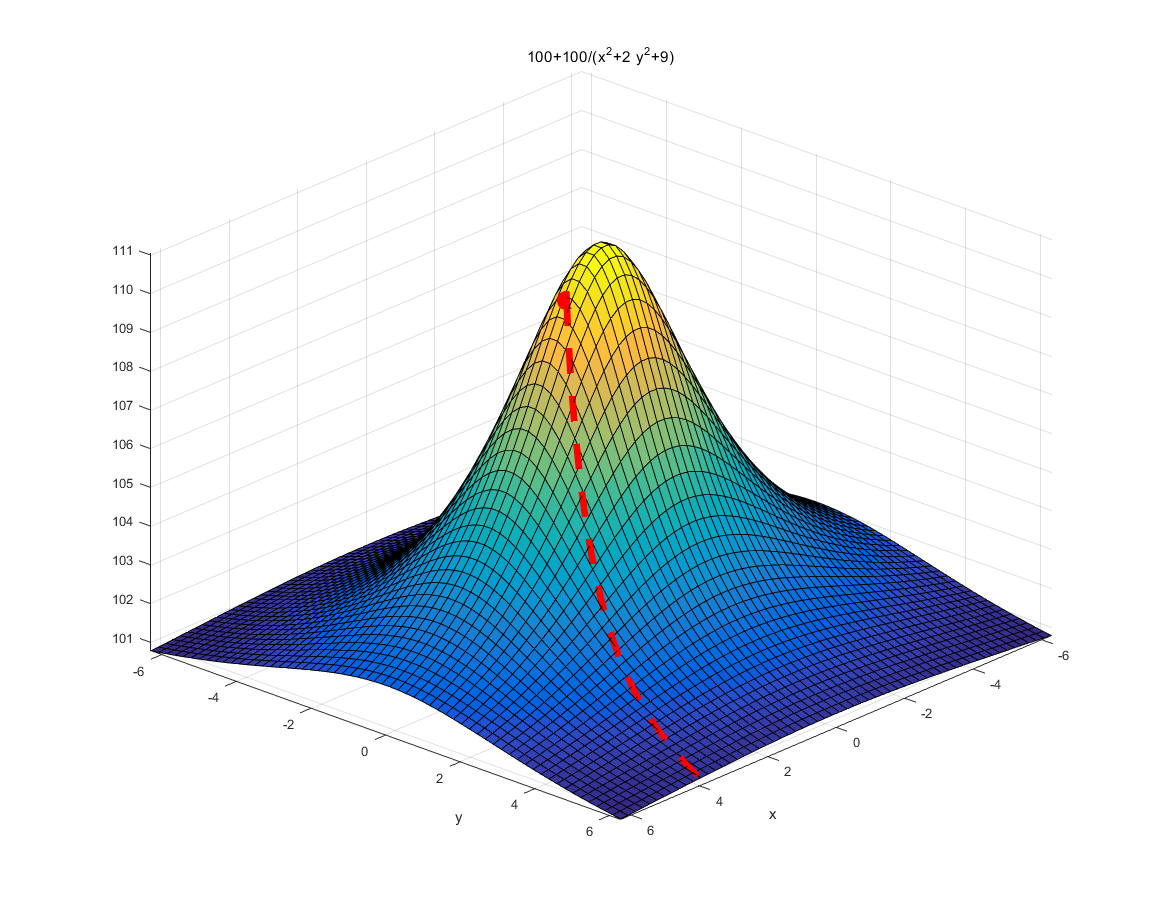
\includegraphics[scale=.2]{image/lec4-1}
\end{center}
\end{exmp}
\end{frame}

\begin{frame}
\begin{thm}
Let $g(x,y,z)$, $f(x,y,z)$ be differentiable functions.
Suppose that $(x_0,y_0,z_0)$ is a local extremal of $f(x,y,z)$ 
restricted the level set $L_c(g)$. 
If $\nabla g(x_0,y_0)\neq\mathbf 0$, 
then there exists $\lambda$ such that
	\[\nabla f(x_0,y_0,z_0)=\lambda\nabla g(x_0,y_0,z_0)\]
\end{thm}

\begin{exmp}
Find the minimal and maximal value of $f(x,y,z)=x^3+y^3+z^3$
on the sphere $x^2+y^2+z^2=1$ on the first octant.
\end{exmp}
\end{frame}

\begin{frame}
\begin{prob}
Find all critical points and classify them
\begin{enumerate}
    \item $\displaystyle f(x,y) = xy + \frac{2}{x} + \frac{2}{y}$
    \item $e^y(x^2+y^2-z^2)$
\end{enumerate}
\end{prob}
\end{frame}

\begin{frame}
\begin{prob}
Find all local extremes of $f(x,y)$ with the give contraints.
\begin{enumerate}
    \item $f(x,y) = 2x+y^2+x^2, 2x^2+y^2 = 2$
    \item $f(x,y,z) = xy+yz, x^2+y^2 = 1, yz = 1$
\end{enumerate}
\end{prob}
\end{frame}

\begin{frame}
\begin{prob}
Find the local extremes of $f(x,y) = x^2+xy+y^2$
on the disk $D = \{(x,y)\mid x^2+y^2\le 1\}$.
\end{prob}
\end{frame}

\begin{frame}
\begin{prob}
Find the point on the graph $xy^2z^3=2$ 
which is the closest to the origin.
\end{prob}
\end{frame}
\end{document}